\documentclass{article}

\usepackage{graphicx}
\usepackage{tikz}
\usepackage{tikzsymbols}
\usetikzlibrary{calc,patterns,shapes.geometric}
\pagestyle{empty}
\usepackage[margin=0pt]{geometry}
\geometry{papersize={14in,12in}}

\def\centerarc[#1](#2)(#3:#4:#5){\draw[#1] ($(#2)+({#5*cos(#3)},{#5*sin(#3)})$) arc (#3:#4:#5);}

\begin{document}
	\begin{figure}
		\centering
		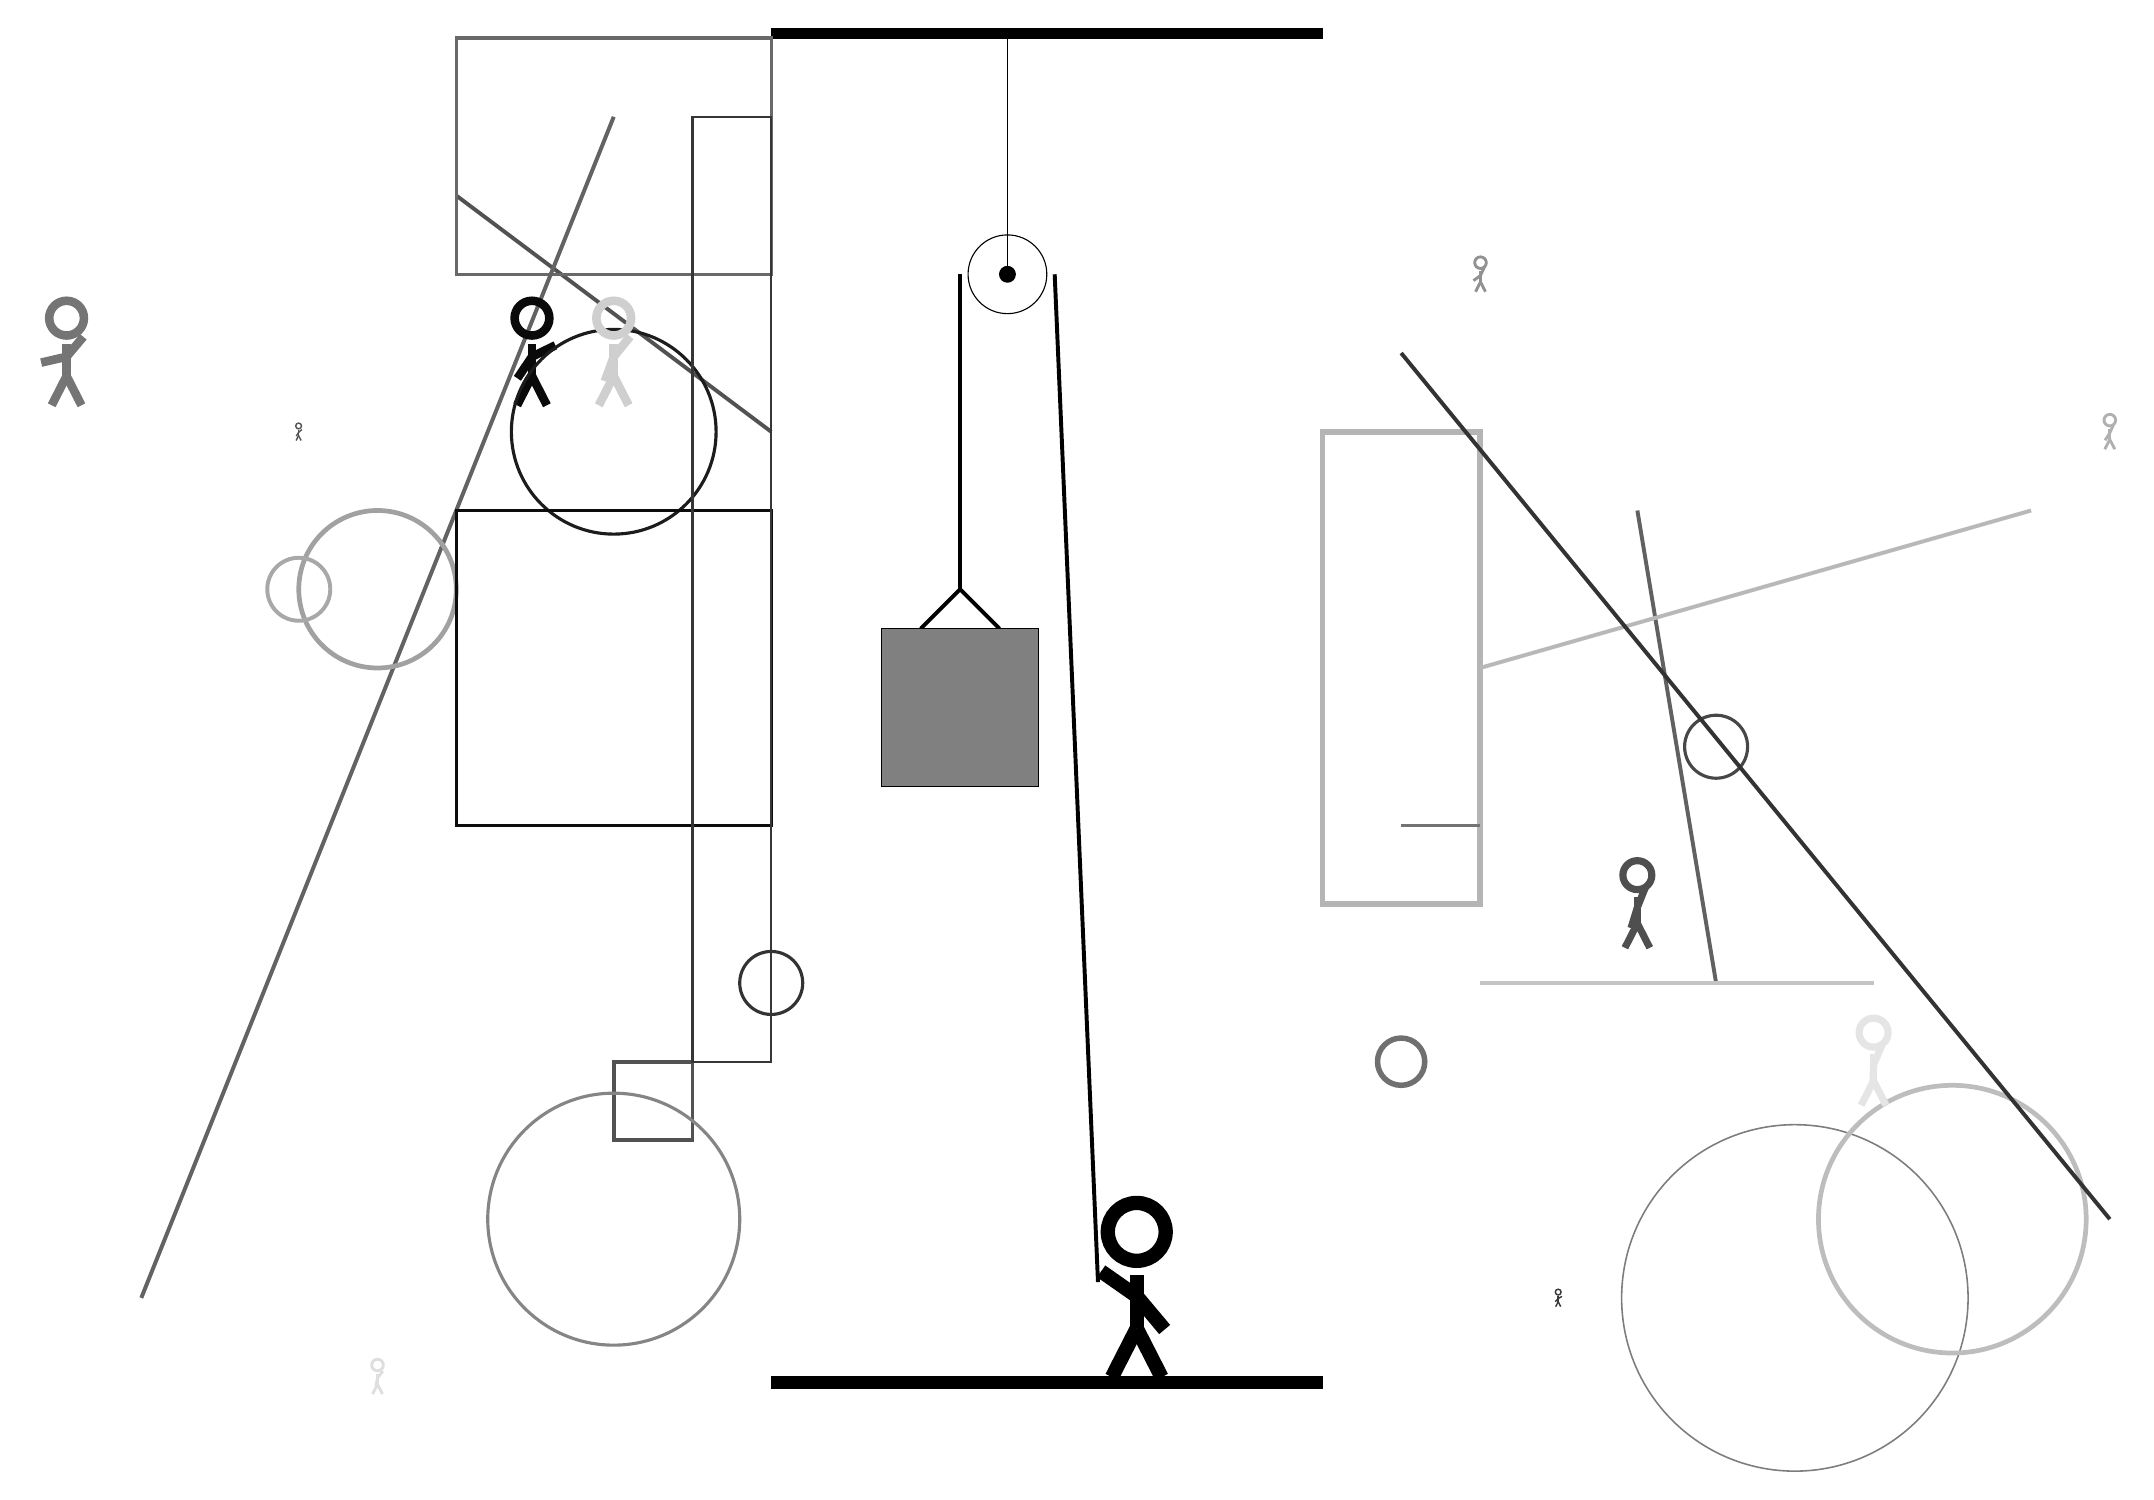
\begin{tikzpicture}
			%%%%% START %%%%%
			
			\draw[fill=black] (-2, 14) rectangle (5, 14.125);
			
			\draw (1, 11) circle (0.5);
			\draw[fill=black] (1, 11) circle (0.1);
			\draw (1, 14) -- (1, 11);
			
			\draw[line width=0.5mm] (-0.1, 6.5) -- (0.4, 7.0) -- (0.9, 6.5);
			\draw[fill=black!50] (-0.6, 6.5) rectangle (1.4, 4.5);
			
			\draw[line width=0.5mm] (0.4, 11) -- (0.4, 7.0);
			\centerarc[line width=0.5mm](1, 11)(0:180:0.6);
			\draw[line width=0.5mm](1.6, 11) -- (2.15, -1.8);
			
			\draw[line width=0.5mm, color=black!62](9, 8) -- (10, 2);
			
			\node[line width=0.4mm, color=black!43] at (7, 11) {\Strichmaxerl[2][36][65]};
			\node[line width=0.6mm, color=black!67] at (-8, 9) {\Strichmaxerl[1][58][41]};
			\draw [line width=0.2mm, color=black!51](11, -2) circle (2.2);
			
			\draw[line width=0.5mm, color=black!68](-6, 12) -- (-2, 9);
			\node[line width=0.2mm, color=black!31] at (15, 9) {\Strichmaxerl[2][57][66]};
			\draw[line width=0.5mm, color=black!23](7, 2) -- (12, 2);
			\draw[line width=0.4mm, color=black!59] (-2, 11) rectangle (-6, 14);
			\draw[line width=0.5mm, color=black!68] (-4, 1) rectangle (-3, 0);
			\draw[line width=0.5mm, color=black!61](-4, 13) -- (-10, -2);
			
			\draw [line width=0.6mm, color=black!37](-7, 7) circle (1.0);
			\draw [line width=0.6mm, color=black!26](13, -1) circle (1.7);
			\node[line width=0.3mm, color=black!96] at (-5, 10) {\Strichmaxerl[6][56][26]};
			
			\node[line width=0.5mm, color=black!54] at (-11, 10) {\Strichmaxerl[6][13][50]};
			\draw [line width=0.4mm, color=black!80](-2, 2) circle (0.4);
			\node[line width=0.7mm, color=black!69] at (9, 3) {\Strichmaxerl[5][73][68]};
			\draw [line width=0.4mm, color=black!48](-4, -1) circle (1.6);
			\draw[line width=0.7mm, color=black!29] (5, 9) rectangle (7, 3);
			\draw [line width=0.7mm, color=black!56](6, 1) circle (0.3);
			\draw[line width=0.5mm, color=black!28](7, 6) -- (14, 8);
			\node[line width=0.7mm, color=black!13] at (-7, -3) {\Strichmaxerl[2][79][52]};
			
			\draw [line width=0.4mm, color=black!89](-4, 9) circle (1.3);
			
			\draw[line width=0.4mm, color=black!95] (-2, 8) rectangle (-6, 4);
			\node[line width=0.6mm, color=black!10] at (12, 1) {\Strichmaxerl[5][88][67]};
			\draw [line width=0.4mm, color=black!72](10, 5) circle (0.4);
			
			\draw[line width=0.3mm, color=black!55] (6, 4) rectangle (7, 4);
			
			\node[line width=0.4mm, color=black!78] at (8, -2) {\Strichmaxerl[1][47][29]};
			\draw[line width=0.5mm, color=black!80](6, 10) -- (15, -1);
			\draw[line width=0.3mm, color=black!79] (-3, 1) rectangle (-2, 13);
			\node[line width=0.7mm, color=black!19] at (-4, 10) {\Strichmaxerl[6][70][51]};
			\draw [line width=0.5mm, color=black!34](-8, 7) circle (0.4);
			
			\node at (2.6, -1.9) {\Strichmaxerl[10][-35][-50]};
			
			\draw[fill=black] (-2, -3) rectangle (5, -3.15);
			
			%%%%% END %%%%%
		\end{tikzpicture}
	\end{figure}	
\end{document}